\documentclass[a4paper, 11pt, finnish]{article}
\usepackage{ucs}
\usepackage[utf8x]{inputenc}
\usepackage[T1]{fontenc}
\usepackage[finnish]{babel}
\usepackage{graphicx}
\usepackage{hyperref}

\setlength{\parindent}{0pt}
\setlength{\parskip}{1ex plus 0.5ex minus 0.2ex}

\author{Topi Talvitie}
\title{frivol: Testausdokumentti}

\begin{document}
\maketitle

Projektissa ainoa varsinaisesti testattava asia oli Voronoi-diagrammikirjasto frivol. Sitä testattiin kolmella tavalla: yksikkötesteillä, suorituskykytestillä ja käsin kokeilemalla frivoldraw-ohjelmalla.

\section*{Yksikkötestit}
Ohjelmaa toteutettaessa jokaiselle uudelle moduulille laadittiin yksikkötestejä, joita ajan myötä täydennettiin (testit löytyvät hakemistosta test, ks. test/README.md jos haluat ajaa testit). Lisäksi lopuksi koko kirjastolle laadittiin yleistesti, joka tarkistaa satunnaissyötteillä.

Yksikkötestejä ei tehty ihan fundamentalistisesti, vaan monesti iso testi testasi montaa asiaa samaa aikaa, tai jotain moduulia ei testattu niin tarkasti koska se tulee testatuksi tarkemmin jonkin toisen sitä moduulia käyttävän moduulin testin yhteydessä. Kuitenkin yhteensä testien kattavuuden pitäisi olla hyvä.

Koska kaikki testit menevät läpi projektin lopuksi, olisi uskottavaa että kirjasto toimisi oikein. Kuitenkin käsin testatessa käy ilmi, etteivät testit saaneet kiinni aivan kaikkia ongelmia.

\section*{Suorituskykytestaus}
Yksikkötesteillä ei testattu ohjelman suorituskykyä, sitä varten kirjoitettiin benchmark-ohjelma perftest (löytyy hakemistosta perftest). Ohjelma arpoo tasaisella satunnaisotannalla pisteitä, ja katsoo kauan frivolilla kestää laskea Voronoi-diagrammi. Ohjelma kokeilee frivolia sekä oletuspolicyllä (binäärikeko ja AVL-puu) että dummypolicyllä (triviaalitoteutukset, operaatiot $O(n)$), ja tallentaa tiedostoon eri pistelukumäärille ajoajat. Tuloksena on seuraavat käyrät (oletuspolicy punaisella, dummypolicy sinisellä, vaaka-akseli pisteiden määrä $n$, pystyakseli ajoaika sekunteina):

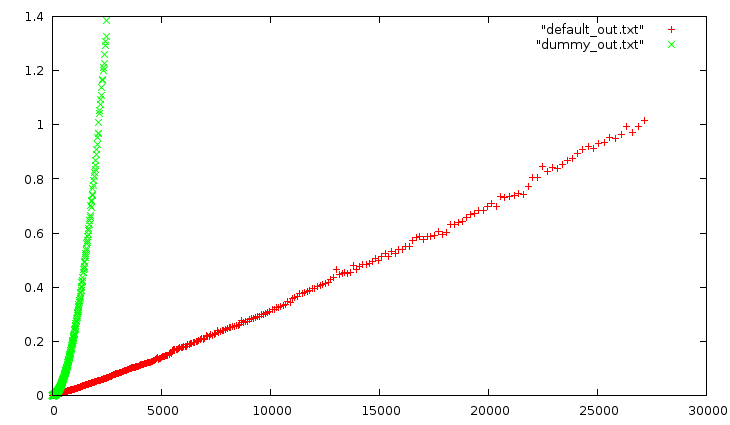
\includegraphics[width=12cm]{perftest.png}

Kuvaajat vastaavat melko hyvin sitä mitä odotettiinkin, eli oletuspolicyllä aikavaativuus $O(n\log n)$ ja dummylla $O(n^2)$. Algoritmilla kuluu 1 sekuntia 25000 pisteen käsittelyyn, eli vakiokerroinkin on mielestäni melko hyvä. 

\section*{Käsin testaus}
Ohjelman testaamiseen käsin toteutettiin frivoldraw-ohjelma (löytyy hakemistosta frivoldraw). frivoldrawissa pisteitä voi raahata ympäriinsä, ja ohjelma näyttää reaaliajassa miten Voronoi-diagrammi muuttuu. Ohjelman ensimäisessä versiossa pisteet ovat aina kokonaislukukoordinaattisia, ja näissä tapauksissa ilmeni välillä ongelmia (ks. Toteutusdokumentti, Puutteet).   Kun testiohjelmaan lisättiin satunnaisperturbaatio, ongelmia ei enää ilmennyt.

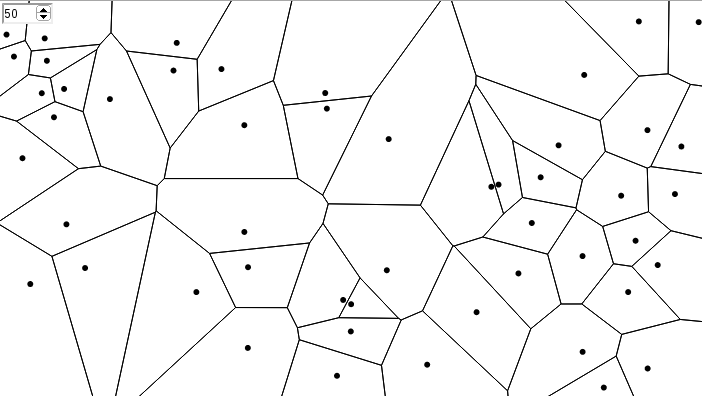
\includegraphics[width=12cm]{frivoldraw.png}

\end{document}
